\subsection{Desarrollo teórico}
Para comenzar el desarrollo teórico, primero definiremos la geometría de la bobina de manera esquemática para entender bien el sistema con el que trabajamos. De manera descriptiva, lo que tenemos es un cilindro hueco de radio \( r_{cext} \) y altura \( h_c \) sobre el cual enrollaremos un hilo de cobre \textbf{\textit{N}} veces. Ligeramente introducido en el cilindro hueco, se encuentra el vástago, que es un cilindro de acero (REFERENCIAR EL ACERO BIEN) de radio \( r_b \) y longitud \( L_b \). La corriente de alimentación será \( i_{dc} \). En la siguiente figura se resume todo en un esquema:

\begin{figure}[h]
    \centering
    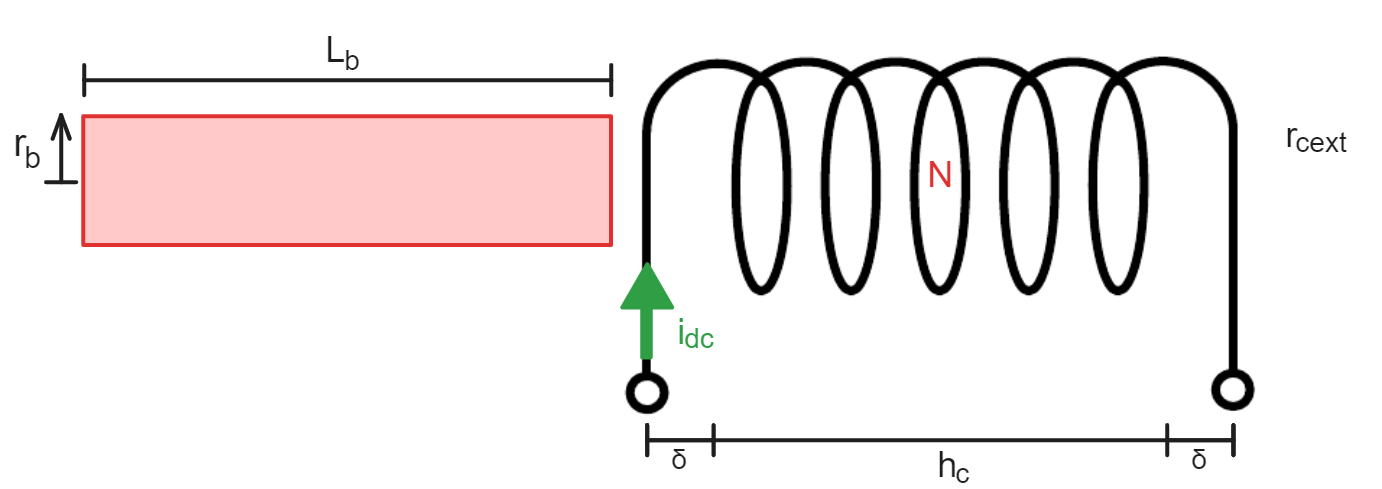
\includegraphics[width=\linewidth]{FigurasMemoria/fig1esquemaGeom.png}
    \caption{Esquema de la bobina y el vástago con sus dimensiones geometrías. Elaboración propia.}
    \label{fig:1} %Para referenciar -> \ref{fig:figNum}
\end{figure}

Los valores iniciales de las dimensiones son:

$$
L_b=0.096m~~~~r_b=0.003045m
\\~\\
h_c=0.05321m~~~~\delta=0.15*h_c~~~~r_{cext}=0.01064m
\\~\\
i_{dc}=3.5A~~N=500
$$

Para empezar el desarrollo, partiremos de la ley integral de Àmpere:

$$
Ni=\oint{\vec{H}\vec{dl}}
$$

Asumiendo un flujo uniforme en la bobina, podemos reescribir:

$$
Ni=Hh_c\to H=\frac{Ni_{dc}}{h_c}
$$

Buscamos ahora una expresión para la densidad de flujo:

$$
B=\mu_0\mu_rH=\mu_0\mu_r\frac{Ni_{dc}}{h_c}
$$

Por otro lado, sabemos que los dipolos magnéticos de un material sentirán una fuerza al verse sometidos a un campo no uniforme de forma: 

$$
\vec F=\nabla(\vec m \cdot\vec B)~~~\forall \vec m=\chi V_{bar}\vec B
$$

Debido a la simplificación realizada, el momento de los dipolos magnéticos y el campo estarán alineados y serán uniformes por lo que podríamos decir:

$$
F=mB=\chi V_{bar}B^2=\chi V_{bar}(\mu_0\mu_r\frac{Ni_{dc}}{h_c})^2
$$

Vamos a realizar la primera estimación de la fuerza en la barra. Introduciendo los datos: 

$$
F\approx53.73~N
$$

Este valor es demasiado alto, y es debido a que tenemos que tener en cuenta que en los extremos de la barra el campo magnético pierde toda uniformidad. Nos centraremos ahora en la búsqueda de esa variación ($\delta B/\delta x$), mientras la fuerza nofs queda:

$$
F=(\mu_0\mu_r\chi\frac{Ni_{dc}}{h_c}V_{bar})\frac{\delta B}{\delta x}
$$

$$
F=\chi V_{bar}B^2
\\~\\
F=(\chi V_{bar} B)\frac{\delta B}{\delta x}
\\~\\
F=(\chi V_{bar}B(x))\frac{\delta B}{\delta x}
\\~\\
\vec{F}=\nabla(\vec m\vec B)~~\forall \vec m=\chi V \vec B;~B=\mu\frac{Ni_{dc}}{h_c}
$$